\section{Неориентированные графы}
\index{Графы!неориентированные} \textbf{Неориентированным графом} называется пара $(V, E)$, где $V$~--- непустое конечное множество вершин графа, $E$~--- совокупность множеств $\{ u, v \}$, где $u, v \in V$.
Элементы~$V$ называются \textbf{вершинами графа}.
Элементы~$E$ называются \textbf{рёбрами графа}.

На рисунках вершины графа изображают точками, а рёбра $e = \{ u, v \}$~--- кривыми, соединяющими точки, которые изображают вершины $u$ и $v$.

Если $e = \{ u, v \} \in E$, то говорят, что:
\begin{itemize}
	\item ребро~$e$ соединяет вершины $u$ и $v$;
	\item $u$ и $v$~--- концы ребра~$e$;
	\item ребро~$e$ инцидентно вершинам $u$ и $v$;
	\item вершины $u$ и $v$ инцидентны ребру~$e$.
\end{itemize}

Вершины называются \textbf{соседними}, или \textbf{смежными}, если их соединяет ребро, иначе~--- \textbf{несоседними}, или \textbf{несмежными}.

\index{deg} Число рёбер, инцидентных вершине~$u$, называется \textbf{степенью вершины} и обозначается $\deg u$.

Если степень вершины равна $0$, то она называется \textbf{изолированной}, а если $1$~--- то \textbf{висячей}.

\begin{lemma}[о~рукопожатиях]
\index{Лемма!о~рукопожатиях}
\begin{equation*}
\sum_{u \in V} \deg u = 2|E|
\end{equation*}
где $(V, E)$~--- граф.
\end{lemma}
\begin{proof}
Достаточно заметить, что каждое ребро увеличивает степени двух некоторых вершин на~$1$.
\end{proof}

\begin{wrapfigure}{r}{0pt}
\noindent
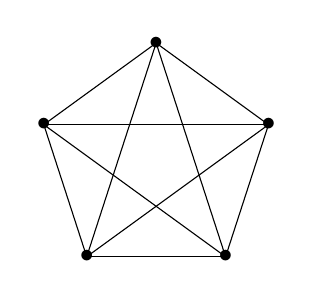
\begin{tikzpicture}[scale=1.5]
\foreach \i in {0, ..., 4}
	\draw (72*\i + 90:1) coordinate (x\i) node {$\bullet$};
\foreach \i in {0, ..., 3}
	\foreach \j in {\i, ..., 4}
		\draw (x\i) -- (x\j);
\end{tikzpicture}
\caption{Граф $K_5$}
\end{wrapfigure}

\index{Петля} Ребро вида $e = \{ u, u \}$ называется \textbf{петлёй}.

Рёбра, инцидентные одним и тем~же вершинам, называются \textbf{кратными}.

Граф называется \textbf{простым}, если он не содержит петель и кратных рёбер.

Граф, в~котором любые две вершины соединены ребром, называется \textbf{полным} и обозначается $K_n$, где $n$~--- число вершин в~нём.

Графы $G_1 = (V_1, E_1)$ и $G_2 = (V_2, E_2)$ называются \textbf{изоморфными}, если существует биекция~$\varphi \colon V_1 \to V_2$ такая, что
$\{ u, v \} \in E_1 \Leftrightarrow \{ \varphi(u), \varphi(v) \} \in E_2$, иначе~--- \textbf{неизоморфными}.
$\varphi$ называется \textbf{изоморфизмом}.

\index{Маршрут} \textbf{Маршрутом} в графе называется последовательность вершин и рёбер вида
$(v_1, e_1, v_2, \ldots, \allowbreak e_k, v_{k+1})$, где $e_i \opbr= \{ v_i, v_{i+1} \}$.

\index{Цепь} Маршрут, в~котором все рёбра различны, называется \textbf{цепью}.

Цепь, в~которой все вершины, за исключением, может быть, первой и последней, различны, называется \textbf{простой}.

Маршрут, в~котором первая и последняя вершины совпадают, называется \textbf{замкнутым}.

\index{Цикл} Замкнутая цепь называется \textbf{циклом}.

Маршрут, соединяющий вершины $u$ и $v$, называется \textbf{$(u, v)$"=маршрутом}.

\begin{lemma}
\label{lemma:walk_contains_simple_chain}
$(u, v)$-маршрут содержит $(u, v)$"=простую цепь.
\end{lemma}
\begin{proof}
Пусть $(u = v_1, e_1, v_2, \ldots, e_k, v_{k+1} = v)$~--- не простая цепь, тогда $\exists i < j \colon v_i = v_j$.
Уберём из маршрута подпоследовательность $(e_i, v_{i+1}, \ldots, e_{j-1}, v_j)$ и получим маршрут, в~котором совпадающих вершин на одну меньше.
Повторяя, получим простую цепь, являющуюся частью данного маршрута.
\end{proof}

\begin{lemma}
\label{lemma:cycle_contains_simple_one}
Любой цикл содержит простой цикл, причём каждая вершина и ребро цикла принадлежат некоторому простому циклу.
\end{lemma}
\begin{proof}
Пусть $(u = v_1, e_1, v_2, \ldots, e_k, v_{k+1} = u)$~--- не простой цикл, тогда $\exists i < j \colon v_i = v_j$.
Уберём из цикла подпоследовательность $(e_i, v_{i+1}, \ldots, e_{j-1}, v_j)$ и получим цикл, в~котором совпадающих вершин на одну меньше.
Повторяя, получим простой цикл, являющийся частью данного цикла.

Заметим, что подпоследовательность $(v_i, e_i, v_{i+1}, \ldots, e_{j-1}, v_j = v_i)$ также является циклом, из которого можно получить простой цикл.
Значит, некоторые вершины и рёбра этой подпоследовательности принадлежат простому циклу, остальные же снова образуют некоторые циклы, из которых можно получить простые.
Продолжая рассуждать таким образом, приходим к выводу, что любая вершина и ребро исходного цикла принадлежат некоторому простому циклу.
\end{proof}
	
\begin{lemma}
\label{lemma:existence_of_simple_cycle}
Если в~графе есть две различные простые цепи, соединяющие одни и те~же вершины, то в~этом графе есть простой цикл.
\end{lemma}
\begin{proof}
Пусть $(u = v_1, e_1, v_2, \ldots, e_n, v_{n+1} = v)$, $(u = v_1', e_1', v_2', \ldots, e_m', v_{m+1}' = v)$~--- простые цепи.
Найдём наименьшее~$i \colon e_i \neq e_i'$, тогда $(v_i, e_i, v_{i+1}, \ldots, e_n, v_{n+1} = v_{m+1}', e_m', \ldots, e_i', v_i' = v_i)$~--- цикл, значит, можно получить простой цикл.
\end{proof}

\subsection{Связность неориентированных графов}
Вершины $u$ и $v$ называются \textbf{связанными}, если существует $(u, v)$"=маршрут, иначе~--- \textbf{несвязанными}.

\index{Графы!связные} Граф называется \textbf{связным}, если в~нём любые две вершины связаны, иначе~--- \textbf{несвязным}.

Граф~$G' = (V', E')$ называется \textbf{подграфом графа~$G = (V, E)$}, если $V' \subseteq V \lAnd E' \subseteq E$.

\index{Компонента связности} \textbf{Компонентой связности графа} называется его максимальный относительно включения связный подграф.

\subsection{Эйлеровы графы}
Цикл, содержащий все рёбра графа, называется \textbf{эйлеровым}.

\index{Графы!эйлеровы} Граф, содержащий эйлеров цикл, называется \textbf{эйлеровым}.

\begin{theorem}
Связный граф эйлеров $\Leftrightarrow$ степени всех вершин чётны.
\end{theorem}
\begin{proof}
\begin{enumerate}
	\item $\Rightarrow$. Пусть в~графе есть эйлеров цикл.
	Выберем вершину~$v_0$ в~этом цикле и начнём обходить его.
	При каждом посещении вершины~$v \neq v_0$ её степень увеличивается на~$2$.
	Т.\,о., если посетить её $k$~раз, то $\deg v = 2k \mult 2$.
	
	Для $v_0$ степень увеличивается на~$1$ в~начале обхода, на~$1$ в~конце обхода и на~$2$ при промежуточных посещениях.
	Т.\,о., её степень чётна.
	
	\item $\Leftarrow$. Пусть степени всех вершин чётны.
	Выберём цепь~$C = (v_0, e_0, v_1, e_1, \ldots, e_{k-1}, v_k)$ наибольшей длины.
	Все рёбра, инцидентные~$v_k$, присутствуют в~этой цепи, иначе её можно было~бы удлинить.
	
	Докажем методом от противного, что $v_0 = v_k$.
	Пусть $v_0 \neq v_k$.
	При прохождении вершины~$v_i = v_k$, $i = 1, 2, \ldots, k - 1$, степень~$v_k$ увеличивается на~$2$.
	Также проходим по ребру~$e_{k-1}$, тогда степень~$v_k$ нечётна.
	Противоречие.
	
	Докажем методом от противного, что $C$ содержит все рёбра.	
	Пусть найдётся ребро~$e = \{ u, v \}$, не входящее в~$C$.
	Возьмём первое ребро~$e' = \{ v_i, v' \}$ из $(v_0, u)$"=маршрута, не входящее в~$C$.
	Тогда цепь~$(v', e', v_i, e_i, \ldots, e_{k-1}, \allowbreak v_k = v_0, \allowbreak e_0, v_1, e_1, \ldots, v_{i-1})$ длиннее, чем~$C$.
	Противоречие.
\end{enumerate}
\end{proof}

\subsubsection{Алгоритмы нахождения эйлерова цикла}
\paragraph{Алгоритм Флёри.}
\index{Алгоритм!Флёри} В качестве текущей вершины выберем произвольную.
\begin{enumerate}
	\item Выбираем ребро, инцидентное текущей вершине.
	Оно не должно быть мостом, если есть другие рёбра, не являющиеся мостами.
	\item Проходим по выбранному ребру и вычёркиваем его.
	Вершина, в~которой теперь находимся,~--- текущая.
	\item Повторяем с шага~1, пока есть рёбра.
\end{enumerate}

\paragraph{Алгоритм объединения циклов.}
\index{Алгоритм!объединения циклов}
\begin{enumerate}
	\item Выбираем произвольную вершину.
	\item Выбираем любое непосещённое ребро и идём по нему.
	\item Повторяем шаг~2, пока не вернёмся в~начальную вершину.
	\item Получили цикл~$C$.
	Если он не эйлеров, то $\exists u \in C, \ e = \{ u, u' \} \colon u' \notin C$.
	Повторяем шаги~2--3, начиная с вершины~$u$.
	Получили цикл~$C'$, рёбра которого не совпадают с рёбрами~$C$.
	Объединим эти циклы и получим новый.
	Повторяем шаг~4.
\end{enumerate}

Цепь называется \textbf{эйлеровым путём}, если она не является циклом и содержит все рёбра графа.

\index{Графы!полуэйлеровы} Граф называется \textbf{полуэйлеровым}, если в~нём есть эйлеров путь.

\begin{theorem}
Связный граф полуэйлеров $\Leftrightarrow$ степени двух вершин нечётны, а остальных~--- чётны.
\end{theorem}
\begin{proof}
\begin{enumerate}
	\item $\Rightarrow$. Пусть в~графе есть эйлеров путь.
	Соединив его концы ребром, получим эйлеров цикл.
	Степени соединённых вершин увеличились каждая на~$1$, значит, они были нечётными, а степени остальных вершин~--- чётными.
	\item $\Leftarrow$. Пусть степени двух вершин нечётны, а остальных~--- чётны.
	Соединим нечётные вершины ребром, тогда можно получить эйлеров цикл.
	Убрав из него добавленное ребро, получим эйлеров путь.
\end{enumerate}
\end{proof}

\subsection{Гамильтоновы графы}
Простой цикл, содержащий все вершины графа, называется \textbf{гамильтоновым}.

\index{Графы!гамильтоновы} Граф называется \textbf{гамильтоновым}, если в~нём есть гамильтонов цикл.

\index{Теорема!Оре}
\begin{theorem}[Оре]
Если в~графе с $n \geqslant 3$~вершинами для любых двух несмежных вершин $u$ и $v$ $\deg u \opbr+ \deg v \opbr\geqslant n$, то граф гамильтонов.
\end{theorem}
\begin{proof}
\begin{enumerate}
	\item Докажем методом от противного, что граф связный.
	Пусть он несвязный, тогда в~нём найдутся хотя~бы две компоненты связности $G_1(V_1, E_1)$ и $G_2(V_2, E_2)$.
	Пусть $u \in V_1$, $v \in V_2$.
	$u$ и $v$ несмежные, тогда
	\begin{equation*}
	\deg u \leqslant |V_1| - 1, \ \deg v \leqslant |V_2| - 1 \Rightarrow \deg u + \deg v \leqslant |V_1| + |V_2| - 2 \leqslant n - 2
	\end{equation*}
	
	Противоречие с условием.
	
	\item Докажем, что граф гамильтонов.
	Выберем цепь~$W = (v_0, e_0, v_1, \ldots, e_{k-1}, v_k)$ наибольшей длины.
	В~ней содержатся все вершины, соседние с~$v_0$ или с~$v_k$.
	Т.\,о., среди вершин $v_1, \ldots, v_k$ находится ровно $\deg v_0$ соседних с~$v_0$ вершин.
	Аналогично для $v_k$.
	
	$\deg v_0 + \deg v_k \geqslant n$, тогда найдутся $v_i$ и $v_{i+1}$ такие, что $v_i$ соседняя с~$v_k$, а $v_{i+1}$~--- с~$v_0$.
	
	Докажем, что $(v_{i+1}, e_{i+1}, \ldots, v_k, e, v_i, e_{i-1}, v_{i-1}, \ldots, e_0, v_0, e', v_{i+1})$~--- гамильтонов цикл, методом от противного.
	Предположим обратное, тогда есть вершина~$u$, не входящая в~цикл, и существует $(v_0, u)$"=маршрут.
	Значит, существует ребро, инцидентное одной из вершин цикла, но не входящее в~него, и можно получить более длинную цепь.
	Противоречие, значит, $G$~--- гамильтонов граф.
\end{enumerate}
\end{proof}

\index{Теорема!Дирака}
\begin{theorem}[Дирака]
\label{th:Dirac}
Если в графе~$G = (V, E)$ с $n \geqslant 3$~вершинами $\forall u \in V \ \deg u \geqslant \frac{n}2$, то граф гамильтонов.
\end{theorem}
\begin{proof}
Пусть $u$, $v$~--- несвязные вершины в~$G$, тогда $\deg u \geqslant \frac{n}2 \lAnd \deg v \geqslant \frac{n}2 \Rightarrow \deg u + \deg v \geqslant n$ $\Rightarrow$ по теореме Оре $G$ гамильтонов.
\end{proof}

Цепь называется \textbf{гамильтоновым путём}, если она не является циклом и содержит все вершины графа.

\index{Графы!полугамильтоновы} Граф называется \textbf{полугамильтоновым}, если в нём есть гамильтонов путь.

\subsection{Планарность графов}
\index{Графы!плоские} \textbf{Плоским} называется граф~$G = (V, E)$ такой, что:
\begin{itemize}
	\item $V \subset \mathbb R^2$;
	\item рёбра~--- кривые, концами которых являются вершины;
	\item различные рёбра не имеют общих точек, за исключением концов.
\end{itemize}

\index{Графы!планарные} \textbf{Планарным} называется граф, изоморфный плоскому.

Если $G$~--- граф и $G'$~--- плоский граф, изоморфный $G$, то $G'$ называется \textbf{укладкой $G$} в~$\mathbb R^2$.

Аналогично можно определить плоский граф в~$\mathbb R^3$, на~сфере и~т.\,д.

\begin{theorem}
Любой граф можно уложить в~$\mathbb R^3$.
\end{theorem}
\begin{proof}
Пусть $G = (V, E)$~--- граф, $V = \{ (1, 0, 0), (2, 0, 0), \ldots, (n, 0, 0) \}$.
Рассмотрим плоскости, проходящие через~$Ox$ и образующие с плоскостью~$Oxy$ углы
$\dfrac\pi2, \dfrac\pi{2\cdot2}, \ldots, \dfrac\pi{2m}$, где $m = |E|$.
В каждой такой плоскости можно провести ровно одно ребро, тогда получим плоский граф, т.\,к. плоскости пересекаются только по прямой~$Ox$.
\end{proof}

\begin{theorem}
Граф укладывается на~плоскость $\Leftrightarrow$ он укладывается на~сферу.
\end{theorem}
\begin{proof}
Пусть плоскость~$z = 0$ касается сферы в точке~$O(0, 0, 0)$, $N$~--- точка на~сфере, диаметрально противоположная точке~$O$.
Для каждой точки сферы, не совпадающей с~$N$, проведём прямую через неё и точку~$N$, которая пересечёт сферу и плоскость, причём любые две из таких прямых имеют единственную общую точку~$N$.
Получим биекцию между точками сферы и точками плоскости, тогда можно построить биекцию между укладками на сфере и укладками на плоскости.
\end{proof}

\begin{center}
\noindent
\shorthandoff{"}
\begin{tikzpicture}[>=stealth]
% рисуем оси
\def\tilt_angle{60}
\draw[->] (0, 0) coordinate["$O$" {below right}] (O) node {$\bullet$}
	+(\tilt_angle:3.5) -- +(\tilt_angle-180:2.5) node[below right] {$x$};
\draw[->] (-4, 0) -- (4.5, 0) node[below] {$y$};
\draw[->] (0, -1.3) -- (0, 4) node[left] {$z$};

% рисуем сферу
\def\radius{1.5}
\draw[name path=sphere] (0, \radius) circle (\radius);

% рисуем плоскость
\def\lenAB{4}
\draw (-4, -1.5) coordinate (A) -- ++(\tilt_angle:\lenAB) coordinate (B);
\draw (A) -- (2, -1.5) coordinate (D) -- ++(\tilt_angle:\lenAB) coordinate (C);
\path[name path=BC] (B) -- (C);
\draw[name intersections={of=BC and sphere, name=i}]
	(B) -- (i-2) (i-1) -- (C);
\draw[dashed] (i-1) -- (i-2);

% рисуем прямую
\draw[dashed] (0, 2*\radius) node[above right] {$N$} node {$\bullet$} -- (-0.6, 0.75) coordinate (point) node {$\bullet$};
\draw (point) -- (-1.15, -1) node {$\bullet$};
\end{tikzpicture}
\shorthandon{"}
\end{center}

Множество на плоскости называется \textbf{линейно связным}, если любые две точки этого множества можно соединить кривой, целиком лежащей в~этом множестве.

\index{Грань} \textbf{Гранью плоского графа~$G = (V, E)$} называется часть множества~$\mathbb R^2 \setminus G$, которая линейно связна и не является подмножеством другого линейно связного множества.

\begin{theorem}[формула Эйлера]
\index{Формула!Эйлера!в~теории графов}
В~плоском связном графе $n - m + f = 2$, где $n, m, f$~--- число вершин, рёбер и граней соответственно.
\end{theorem}
\begin{proof}
Рассмотрим остов данного графа.
В~нём $n$~вершин, $n - 1$~рёбер и $1$~грань.
Формула Эйлера верна для него: $n - (n - 1) + 1 = 2$.

Добавим $1$~ребро данного графа, тогда оно разобьёт одну грань на две, т.\,е. число граней увеличится на~$1$.
Формула Эйлера верна для полученного графа.
Повторяя $m - (n - 1)$~раз, получим исходный граф, для которого формула Эйлера верна.
\end{proof}

\begin{theorem}
\label{th:property_of_planarity_of_graph}
Пусть $G$~--- планарный граф с $n \geqslant 3$~вершинами и $m$~рёбрами. Тогда $m \leqslant 3n - 6$.
\end{theorem}
\begin{proof}
При $m = 2$ неравенство выполняется.

Пусть в~графе $f$~граней, $m_i$~--- число рёбер в~границе $i$-й грани.
Тогда $m_i \geqslant 3$, $\sum\limits_{i=1}^f m_i \geqslant 3f$.
С~другой стороны, $\sum\limits_{i=1}^f m_i \leqslant 2m$, т.\,к. каждое ребро является границей для не более чем $2$ граней.
По формуле Эйлера $n - m + f = 2 \Leftrightarrow f = m + 2 - n$.
Получим:
\begin{equation*}
2m \geqslant 3f \Leftrightarrow 2m \geqslant 3m + 6 - 3n \Leftrightarrow m \leqslant 3n - 6
\end{equation*}
\end{proof}

\begin{consequent}
Планарный граф~$G = (V, E)$ содержит хотя~бы одну вершину со~степенью, не большей~$5$.
\end{consequent}
\begin{proofcontra}
Пусть $\forall v \in V \ \deg v \geqslant 6$, $|V| = n$, $|E| = m$, тогда
$m \opbr= \frac12 \sum\limits_{v \in V} \deg v \opbr\geqslant 3n$.
Имеем:
\begin{equation*}
3n \leqslant m \leqslant 3n - 6 \Rightarrow 0 \leqslant -6
\end{equation*}

Противоречие.
\end{proofcontra}

\begin{theorem}
Графы $K_5$ и $K_{3,3}$ не планарные.
\end{theorem}
\begin{proof}
\begin{itemize}
	\item Рассмотрим $K_5$.
	Для него $n = 5$, $m = 10$.
	Тогда $m \leqslant 3n - 6 \Leftrightarrow 10 \leqslant 9$.	
	Неверно, значит, $K_5$ не планарен.
	\item Рассмотрим $K_{3,3}$.
	Пусть он планарный.
	В~нём самый короткий цикл имеет длину~$4$.
	Тогда рассуждениями, аналогичными рассуждениям при доказательстве теоремы~\ref*{th:property_of_planarity_of_graph}, получим
	\begin{equation*}
	2m \geqslant 4f \Leftrightarrow 2m \geqslant 4m + 8 - 4n \Leftrightarrow m \leqslant 2n - 4
	\end{equation*}
	
	Для $K_{3,3}$ $n = 6$, $m = 9$, тогда $9 \leqslant 8$.
	Неверно, значит, $K_{3,3}$ не планарен.
\end{itemize}
\end{proof}

Граф~$G' = (V', E')$ получается \textbf{подразбиением ребра~$e = \{ u, v \}$} графа~$G = (V, E)$, если:
\begin{itemize}
	\item $V' = V \cup \{ u' \}$;
	\item $E' = (E \setminus \{ e \}) \cup \{ \{ u, u' \}, \{ v, u' \} \}$.
\end{itemize}

\index{Графы!гомеоморфные} Графы $G$ и $G'$ \textbf{гомеоморфны}, если они изоморфны графам, получающимся подразбиениями рёбер одного и того~же графа.

\begin{theorem}[Понтрягина"--~Куратовского]
\index{Теорема!Понтрягина"--~Куратовского}
Граф~$G$ планарен $\Leftrightarrow$ он не содержит подграфов, гомеоморфных $K_5$ или $K_{3,3}$.
\end{theorem}
\begin{proof}
\begin{enumerate}
	\item $\Rightarrow$. Очевидно, что подграф планарного графа планарен.
	Если $G$~--- планарный граф, содержащий подграф $G'$, гомеоморфный $K_5$ или $K_{3,3}$, то $G'$ тоже планарный, значит, $K_5$ или $K_{3,3}$ планарен, т.\,к. подразбиение ребёр не влияет на планарность.
	Противоречие, значит, $G$ не планарен.
	\item $\Leftarrow$. Доказательство слишком сложно, поэтому здесь не приводится.
\end{enumerate}
\end{proof}

\subsection{Деревья}
\index{Лес} Граф без циклов называется \textbf{лесом}.

\index{Дерево} Связный лес называется \textbf{деревом}.

\index{Мост} Ребро называется \textbf{мостом}, если при его удалении увеличивается число компонент связности.

\begin{statement}
\label{st:criterion_of_bridge_in_graph}
Ребро~--- мост $\Leftrightarrow$ оно не содержится в~цикле.
\end{statement}
\begin{proof}
\begin{enumerate}
	\item $\Leftarrow$.
	Пусть ребро $e$ содержится в цикле $W = (v_0, e_0, \ldots, u, e, v, \ldots, v_k)$, $u'$ и $v'$~--- связные вершины.
	\begin{enumerate}
		\item Если в~$(u', v')$"=маршруте нет ребра~$e$, то при его удалении из графа $u'$ и $v'$ останутся связными.
		\item Пусть $(u' = v_0', e_0', \ldots, u, e, v, \ldots, e_m', v_m' = v')$~--- маршрут, соединяющий $u'$ и $v'$, тогда при удалении $e$ из графа $u'$ и $v'$ соединяет маршрут
		$(u' = v_0', e_0', \ldots, u, \ldots, e_0, v_0 = v_k, e_{k-1}, \ldots, v, \ldots, e_m', v_m' = v')$.
	\end{enumerate}
	
	\item $\Rightarrow$.
	Пусть $e = \{ u, v \}$ не является мостом, тогда $u$, $v$ лежат в~одной компоненте связности.
	Удалим $e$ из графа.
	Число компонент связности не изменится, значит, $u$ и $v$ также лежат в~одной компоненте связности, т.\,е. существует цепь, соединяющая $u$ и $v$: $(u = v_0, e_0, \ldots, e_{k-1}, v_k = v)$.
	Тогда в~исходном графе существует цикл $(u = v_0, e_0, \ldots, e_{k-1}, v_k = v, e, u)$.
\end{enumerate}
\end{proof}

\begin{theorem}
Следующие утверждения о графе~$G = (V, E)$ с~$n$ вершинами эквивалентны:
\begin{enumerate}
	\item $G$~--- дерево.
	\item $G$ связный и каждое его ребро~--- мост.
	\item $G$ связный и имеет $n - 1$~ребро.
	\item $G$ не содержит циклов и имеет $n - 1$~ребро.
	\item Любые две вершины графа~$G$ соединены ровно одной простой цепью.
	\item $G$ не содержит циклов и добавление ребра приводит к появлению ровно одного цикла.
\end{enumerate}
\end{theorem}
\begin{proof}
\begin{itemize}
	\item 1 $\Rightarrow$ 2.
	Связность следует из определения дерева.
	
	В~силу утверждения~\ref*{st:criterion_of_bridge_in_graph} каждое ребро~--- мост.
	
	\item 2 $\Rightarrow$ 3.
	Связность следует из предположения.
	
	Докажем методом математической индукции, что в~графе $n - 1$~ребро.
	\indbase Для $n = 1, 2$ очевидно.
	\indstep Пусть утверждение верно для чисел, меньших $n$.
	Возьмём мост~$e$ и удалим его.
	Получим две компоненты связности $G_1 = (V_1, E_1)$, $G_2 = (V_2, E_2)$.
	По предположению индукции $|E_1| = |V_1| - 1$, $|E_2| = |V_2| - 1$.
	Тогда в~исходном графе рёбер $|E_1| + |E_2| + 1 = |V_1| + |V_2| - 1 = n - 1$. \indend
	
	\item 3 $\Rightarrow$ 4.
	$G$ имеет $n - 1$~ребро по предположению.
	
	Докажем методом математической индукции, что $G$ не содержит циклов.
	\indbase Для $n = 1, 2$ очевидно.
	\indstep Пусть утверждение верно для чисел, меньших $n$.
	Докажем методом от противного, что в~графе есть вершина степени~$1$.
	Пусть
	\begin{equation*}
	\forall u \in V \ \deg u \geqslant 2 \Rightarrow 2|E| = \sum_{u \in V} \deg u \geqslant 2n \Rightarrow n - 1 = |E| \geqslant n \Rightarrow -1 \geqslant 0
	\end{equation*}
	Противоречие, значит, в~графе найдётся вершина степени~$1$.
	
	Удалим её и инцидентное ей ребро.
	Полученный граф содержит $n - 1$~вершину и удовлетворяет утверждению~3.
	По предположению индукции он не содержит циклов, тогда и исходный граф не содержит циклов. \indend
	
	\item 4 $\Rightarrow$ 5.
	
	Пусть в~графе $k$~компонент связности: $G_1 = (V_1, E_1)$, $G_2 = (V_2, E_2)$, \ldots, $G_k = (V_k, E_k)$.
	Они не содержат циклов по предположению, тогда они являются деревьями.
	\begin{equation*}
	|E_1| = |V_1| - 1 \lAnd |E_2| = |V_2| - 1 \lAnd \ldots \lAnd |E_k| = |V_k| - 1 \lAnd 
	n - 1 = |E_1| + \ldots + |E_k| = n - k \Rightarrow k = 1
	\end{equation*}
	Значит, граф связный.
	
	Пусть существуют вершины $u$ и $v$ такие, что их соединяют две простые цепи, тогда по лемме~\ref{lemma:existence_of_simple_cycle} в~графе есть цикл, что противоречит предположению.
	Значит, эти вершины соединены ровно одной простой цепью.
	
	\item 5 $\Rightarrow$ 6.
	
	Докажем методом от противного, что в~графе нет циклов.
	Предположим, что есть цикл $(v_0, e_0, v_1, \ldots, v_k = v_0)$, тогда есть две простые цепи $(v_0, e_0, \ldots, v_{k-1})$ и $(v_{k-1}, e_k, v_k = v_0)$, соединяющие $v_0$ и $v_{k-1}$, что противоречит предположению.
	
	Докажем, что добавление ребра приводит к появлению ровно одного цикла.
	Рассмотрим несоседние вершины $u$ и $v$.
	По предположению есть цепь $(u = v_0, e_0, \ldots, v_k = v)$, соединяющая их.
	Тогда, добавив $e = \{ u, v \}$, получим цикл $(u = v_0, e_0, \ldots, v_k = v, e, u)$.
	
	Пусть есть $2$~цикла, соединяющих $u$ и $v$.
	Удалим $e$, тогда один цикл останется.
	Получим исходный граф, в~котором не должно быть циклов.
	Противоречие.
	
	\item 6 $\Rightarrow$ 1.
	
	Докажем связность методом от противного.
	Рассмотрим несвязные вершины $u$ и~$v$.
	Соединим их и по~предположению получим цикл $(v_0, e_0, \ldots, u, e, v, \ldots, e_{k-1}, v_k = v_0)$.
	Тогда в~исходном графе $(u, \ldots, e_0, v_0 = v_k, \allowbreak e_{k-1}, \ldots, v)$~--- $(u, v)$"=маршрут.
	Противоречие.
\end{itemize}
\end{proof}

В~ходе доказательства было получено, что в~связном графе с $n$~вершинами и $n - 1$~рёбрами существует висячая вершина.
Т.\,к. доказано, что такой граф является деревом, то верно следующее утверждение.
\begin{statement}
В~дереве существует висячая вершина.
\end{statement}

\begin{statement}
Если в лесу $n$~вершин, $m$~рёбер и $k$~компонент связности, то $m = n - k$.
\end{statement}
\begin{proof}
Пусть $n_1, \ldots, n_k$~--- число вершин в каждой компоненте связности, тогда
\begin{equation*}
m = (n_1 - 1) + (n_2 - 1) + \ldots + (n_k - 1) = n - k
\end{equation*}
\end{proof}

\subsection{Остовы}
\index{Остов} \textbf{Остовом графа $G = (V, E)$} называется его подграф~$G' = (V', E') \colon V = V' \lAnd G'$~--- дерево.

\begin{statement}
Любой связный граф содержит остов.
\end{statement}

\begin{statement}
Если граф не является деревом, то в~нём несколько остовов.
\end{statement}

Пусть $G = (V, E)$~--- граф.

\index{Вес} \textbf{Весом} называется функция~$\alpha \colon E \to \mathbb R^+$.

\textbf{Весом ребра}~$e \in E$ называется $\alpha(e)$.

\textbf{Весом графа} называется $\sum\limits_{e \in E} \alpha(e)$.

Пусть дан граф~$G = (V, E)$, $n = |V|$ и весовая функция $\alpha \colon E \to R^+$, и необходимо найти остов наименьшего веса $T = (V, P)$.

\subsubsection{Алгоритм Краскала}
\index{Алгоритм!Краскала}
\begin{enumerate}
	\item[1.] Выбираем ребро~$e \in E$ с наименьшим весом: $P_1 = \{ e \}$, $T_1 = (V, P_1)$.
	\item[i.] Выбираем ребро~$e \in E$ с наименьшим весом такое, что $e \notin P_i$ и добавление этого ребра не приводит к образованию цикла в~$T$: $T_{i+1} = (V, P_i \cup \{ e \})$.
\end{enumerate}

$T_n$~--- искомый остов.
\begin{proof}[корректности]
	Пусть $T = (V, P)$~--- построенный остов, где
	$P = \{ e_1, e_2, \ldots, e_{n-1} \}$, $e_1, e_2, \ldots, \allowbreak e_{n-1}$~--- рёбра в~порядке их добавления в~остов, а также $D = (V, M)$~--- другой остов, где
	$M = \{ e_1', e_2', \ldots, e_{n-1}' \}$, $e_1', e_2', \ldots, e_{n-1}'$~--- рёбра в~порядке неубывания их весов.
	
	Если $T \neq D$, то пусть $i$~--- наименьшее число такое, что $e_i \neq e_i'$.
	$e_i'$ не входит в~$T$, значит, оно образует цикл с рёбрами в~$T$, выбранными ранее, тогда вес этих рёбер не больше $\alpha(e_i')$.
	Выберем из них ребро~$e$ такое, что при добавлении его в~$D$ образуется цикл.
	Пусть $D_1 = (V, M \cup \{ e \} \setminus \{ e_i' \})$.
	Этот граф~--- остов, причём вес~$D_1$ не больше веса~$D$ и у~$T$ и $D_1$ на~$1$ общее ребро больше, чем у~$T$ и $D$.
	Повторяя, получим $D_k = T$.
	Значит, вес построенного остова не превосходит веса любого другого остова.
\end{proof}

\subsubsection{Алгоритм Прима}
\index{Алгоритм!Прима}
Строится последовательность деревьев $S_1 \subset S_2 \subset \ldots \subset S_n = T$.
\begin{enumerate}
	\item[1.] Выбираем произвольную вершину~$v$.
	$S_1 = (\{ v \}, \varnothing)$.
	\item[i.] Пусть построено $S_{i-1} = (V_{i-1}, E_{i-1})$.
	Находим ребро~$e = \{ u, v_{i-1} \} \in E$, где $u \in V_{i-1}$, $v_{i-1} \notin V_{i-1}$, наименьшего веса, добавление которого не приводит к образованию цикла: $S_i = (V_{i-1} \cup \{ v_{i-1} \}, E_{i-1} \cup \{ e \})$.
\end{enumerate}

$S_n$~--- искомый остов.

\subsection{Помеченные деревья}
\index{Дерево!помеченное} Дерево с $n$~вершинами, которым сопоставлены числа~$1, \ldots, n$, называется \textbf{помеченным}.

\index{Код Прюфера} Каждому помеченному дереву можно взаимнооднозначно сопоставить последовательность из $n - 2$~чисел от $1$ до $n$, называемую \textbf{кодом Прюфера}.
Алгоритм построения кода Прюфера для помеченного дерева~$G = (V, E)$:
\begin{enumerate}
	\item Выбираем висячую вершину~$v$ с наименьшим номером.
	\item Добавляем номер вершины, смежной с~$v$, в~код.
	\item Удаляем~$v$ и ребро, инцидентное $v$, из дерева.
	\item Повторить, начиная с шага~1, $n - 2$~раза.
\end{enumerate}

\begin{statement}
Различным помеченным деревьям соответствуют различные коды Прюфера.
\end{statement}
\begin{proofmathind}
	\indbase При $n = 3$ легко проверить.
	\indstep Пусть утверждение верно при $n$, $G = (V, E)$ и $G' = (V', E')$~--- различные помеченные деревья с $n + 1$~вершинами в~каждом.
	Если в $G$ и $G'$ вершины с наименьшим номером смежны с вершинами с одинаковыми номерами, то выполняем шаг построения кода, тогда оставшиеся деревья различны, значит, по предположению индукции у них различные коды. \indend
\end{proofmathind}

Алгоритм построения дерева по коду $A_0 = (a_0, \ldots, a_{n-3})$:

Пусть $B_0 = \{ 1, \ldots, n \}$.
\begin{enumerate}
	\item Находим наименьшее $b \in B_i \colon b \notin A_i$.
	Тогда в~дереве есть ребро $\{ b, a_i \}$: $A_{i+1} = A_i \setminus \{ a_i \} \lAnd B_{i+1} = B_i \setminus \{ b \}$.
	\item Повторяем шаг~1 $n - 2$~раз.
	Получим $B_{n-2} = \{ b', b'' \}$, значит, в~дереве есть ребро~$\{ b', b'' \}$.
\end{enumerate}

Докажем, что указанный алгоритм по коду из $n$~чисел строит дерево.
\begin{proofmathind}
	\indbase При $n = 1$ легко проверить.
	\indstep Рассмотрим графы $T_1, \ldots, T_{n-1}$, полученные в~процессе построения дерева.
	$T_1$ не содержит циклов.
	$T_2$ получается из $T_1$ либо добавлением новой вершины, либо добавлением моста, что не приводит к появлению цикла.	
	По индукции получим, что $T_{n-1}$ не содержит циклов и содержит $n$~вершин и $n - 1$~ребёр, значит, $T_{n-1}$~--- дерево.
	\indend
\end{proofmathind}

\index{Теорема!Кэли}
\begin{theorem}[Кэли]
Количество неизоморфных помеченных деревьев с $n$~вершинами равно~$n^{n-2}$.
\end{theorem}